\documentclass[letterpaper, 10 pt, conference]{ieeeconf}
\IEEEoverridecommandlockouts 
\overrideIEEEmargins
\usepackage[utf8]{inputenc}
\usepackage[T1]{fontenc}
\usepackage{enumitem}
\usepackage{amsmath}
\usepackage{listings}
\usepackage{graphicx}


\title{\LARGE \bf Aplicación de Redes Neuronales para el Diagnostico de Diabetes Mellitus}

\author{German López Rodrigo\\}

\begin{document}

\maketitle
\thispagestyle{empty}
\pagestyle{empty}

\section{Resumen}
El presente artículo pretende mostrar al lector de cualquier área, las bondades de utilizar redes neuronales para la predicción de datos. Para ello se recurre al desarrollo de un caso aplicado a la asistencia en el diagnóstico de diabetes mellitus, el objetivo es que mediante los datos médicos recopilados de una persona podamos diagnosticar si muestra signos de diabetes de acuerdo con los criterios de la Organización Mundial de la Salud.

\section{Palabras clave}
Redes Neuronales, Aprendizaje Automático, Diabetes Mellitus, Algoritmo predictivo.

\section{Descripción del problema}

La diabetes mellitus es una enfermedad que en las últimas décadas ha mostrado el alto grado de incidencia y prevalencia en los sistemas de salud publica a nivel mundial, especialmente en el continente Americano. Según estimaciones actuales, en México la población aproximada de personas con diabetes asciende entre 10 y 15 millones de personas y ocasiona 80 mil muertes anuales, afectando a todas las clases sociales, principalmente a la población de bajos recursos económicos asentada en las áreas urbanas. \cite{1}. Por este motivo, es importante implementar nuevos algoritmos y técnicas que sean capaces de proporcionar un diagnóstico temprano sobre las pacientes con el fin de que sean tratados de forma eficiente y rápida.\\

\begin{itemize}[leftmargin=*]
    \item \textbf{Pregunta de investigación}
    \\¿Qué información registrada de las personas en el sector salud se puede utilizar para diagnosticar a una persona de Diabetes Mellitus?\\
    
    \item \textbf{Objetivo}
    \\Determinar una Red Neuronal que ayude en la detección oportuna de Diabetes Mellitus.\\

    \item \textbf{Fuente de Datos}
    \\Diabetes \cite{dataset:2019} es una fuente de datos que consta de 768 observaciones y 8 características numéricas. Esta fuente de datos es la que será utilizada para cumplir con el objetivo principal del presente artículo de investigación. Cabe aclarar que la fuente de datos fue dividida en dos conjuntos: un conjunto de 500 observaciones para construir la red neuronal y otro conjuntó de 268 observaciones para realizar las pruebas de la red neuronal.\\
\end{itemize}

\section{Introducción}

La diabetes es una enfermedad sistémica, crónico-degenerativa, de carácter heterogéneo, con grados variables de predisposición hereditaria y con participación de diversos factores ambientales, caracterizada por el aumento de los niveles de glucosa sanguínea (hiperglucemia), causada por un defecto (completo o no) en la secreción o acción de la insulina y o resistencia a la acción de la insulina producida por el propio cuerpo. Actualmente México ocupa el noveno lugar de diabetes en el mundo, 13 de cada 100 muertes son provocadas por la diabetes \cite{2}. El diagnóstico temprano se realiza a toda mujer mayor de 25 años mediante un  examen de hemoglobina A1c y una prueba de tolerancia a la glucosa. De esta forma, con el fin de poder crear un método distinto y más eficaz comparado con los estudios de laboratorio, el presente trabajo propone utilizar una red neuronal para la detección temprana de diabetes mellitus.\\

Una red neuronal es un modelo computacional vagamente inspirado en el comportamiento observado en su homólogo biológico. Consiste en un conjunto de unidades, llamadas neuronas artificiales, conectadas entre sí para transmitirse señales. La información de entrada atraviesa la red neuronal (donde se somete a diversas operaciones) produciendo unos valores de salida. Cada neurona está conectada con otras a través de arcos dirigidos (modelando la conexión con axón $\rightarrow$ dendritas), donde cada arco j $\rightarrow$ i sirve para propagar la salida de la neurona j (notada $a_j$) que servirá como una de las entradas para la neurona i. Además cada arco j $\rightarrow$ i tiene un peso numérico asociado $w_{ji}$ que determina la fuerza y el signo de la conexión (simulando la sinapsis).\\

\begin{figure}[htbp]
\centerline{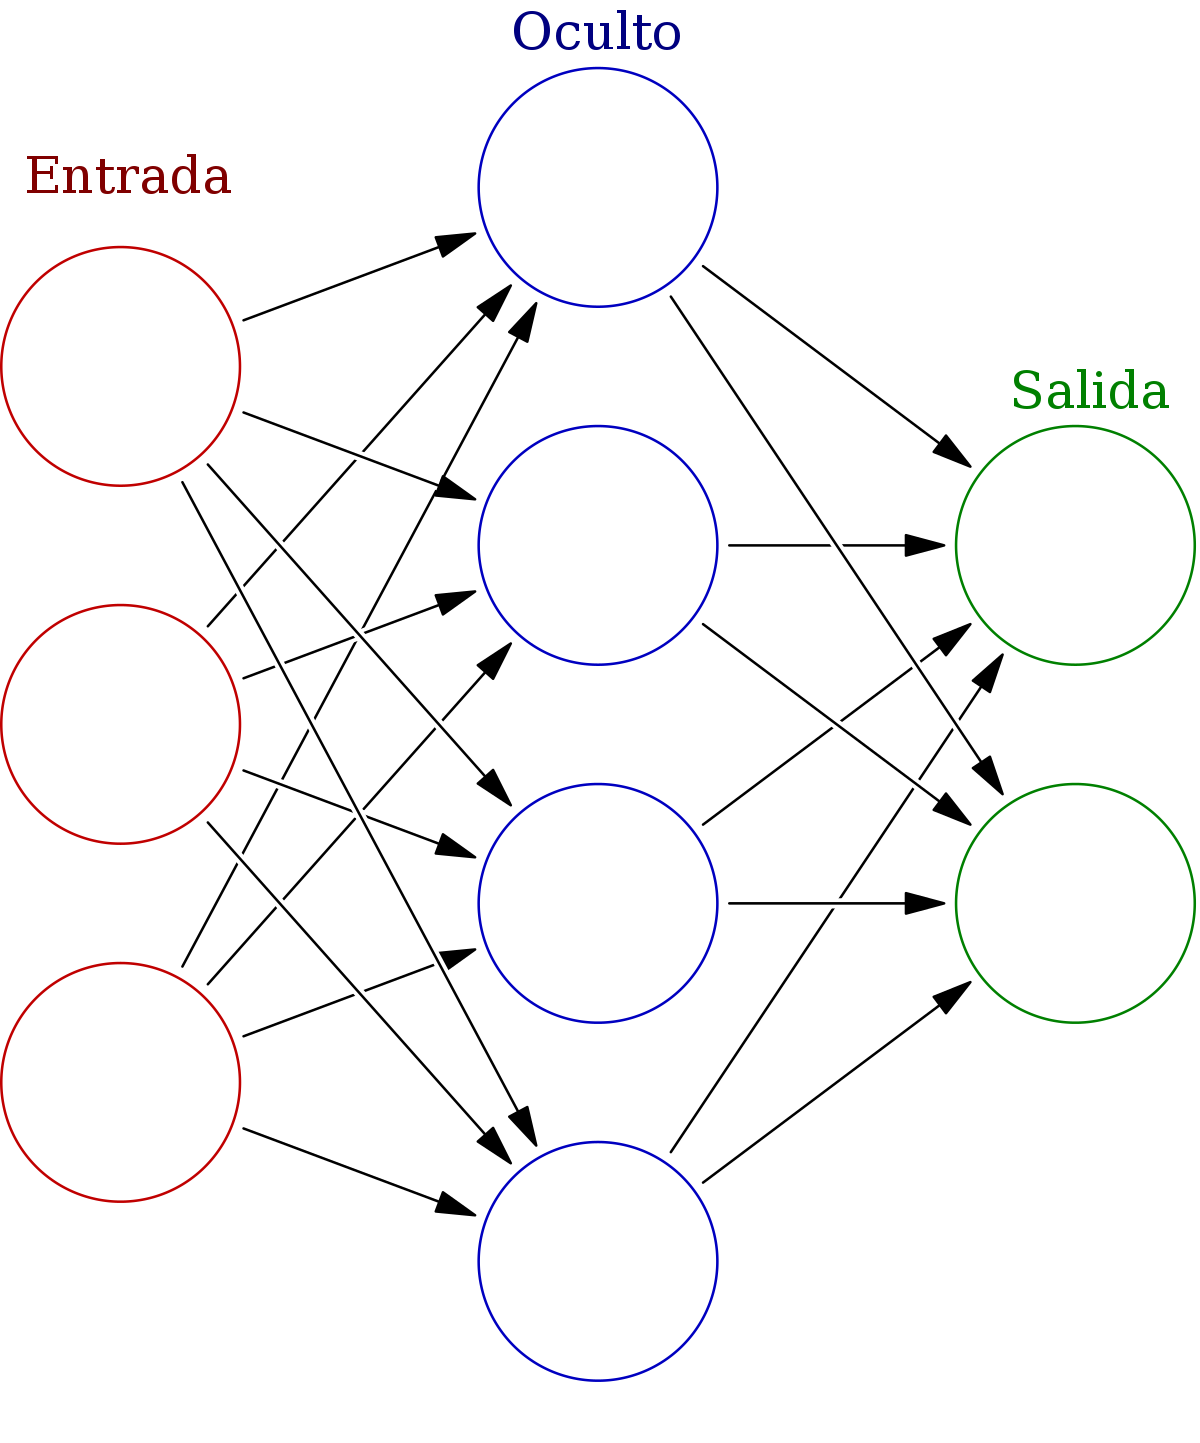
\includegraphics[width=0.25\textwidth]{Images/RN}}
\caption{Red Neuronal}
\label{fig:1}
\end{figure}

\section{DESARROLLO DE CONTENIDO}

Para poder diagnosticar si una persona muestra signos de diabetes mellitus, se utilizó una red neuronal con una capa de entrada con 8 neuronas, 3 capas ocultas con 13 neuronas cada una y una capa de salida con una neurona. El diagnóstico se estableció como la variable dependiente la cual estaría en función de los siguientes datos médicos: número de veces embarazada, concentración de glucosa en plasma a 2 horas en una prueba de tolerancia a la glucosa oral, presión arterial diastólica, grosor del pliegue de tríceps, insulina sérica de 2 horas, índice de masa corporal, función de pedigrí de la diabetes y los años de edad.\\

La red neuronal es construida a partir de un algoritmo desarrollado en lenguaje Python, a continuación se explica el proceso que sigue el algoritmo para la construcción de la red neuronal. El algoritmo consta de tres etapas principales:\\

\begin{itemize}[leftmargin=*]
    \item \textbf{Etapa de Construcción}
    \\ En esta etapa el algoritmo se encarga de construir la red neuronal para esto el primer paso que realiza el algoritmo es ensamblar y unir cada capa de la red neuronal con la finalidad de tener en memoria la red neuronal. Para la capa de entrada el algoritmo se encarga de crear una neurona respecto a cada variable de entrada con el objetivo de poder propagar la entrada a cada neurona de la primera capa oculta. En estas neuronas los pesos iniciales son la unidad y el número de salidas (Axon's) corresponde al número de neuronas que contendrá la primera capa oculta. Para cada una de las capas ocultas el algoritmo se encarga de crear el número de neuronas que contendra cada capa oculta, para cada neurona se generan unos pesos iniciales aleatorios y se definen el número de conexiones de salida (Axon's). Por último el algoritmo se encarga de crear la única neurona de la capa de salida, la salida de esta neurona corresponde al valor final de la red neuronal. Cabe aclarar que para cada neurona se considera una entrada extra denomminada umbral y que la función de activación que se utiliza es la sigmoide.
    
    \begin{equation}
        \sigma(x) = \frac{1}{1+e^{-x}}
    \end{equation}
    
    \begin{equation}
        \sigma(x)' = \sigma(x)(1-\sigma(x))
    \end{equation}

    \item \textbf{Etapa de Procesamiento de Datos}
    \\En esta etapa el algoritmo se encarga de realizar el entrenamiento de la red neuronal, para esto se realiza una propagación hacia adelante de cada uno los valores entrada con el objetivo de obtener el valor generado por la red neuronal, debido a que los pesos iniciales no pueden generar los valores esperados correctos, el algoritmo se encarga de ir calculando el error entre el valor esperado y el valor obtenido de la red neuronal con la finalidad de ir actualizando los pesos de la red neuronal hasta que el error cuadrático se encuentre por debajo de una cota prefijada.\\\\ Para la actualización de los pesos se utiliza el algoritmo de retropropagación el cual nos permite ir propagando el error hacia atrás con la finalidad de poder ir actualizando de forma equitativa los pesos de cada neurona pertenecientes cada capa de la red neuronal. Lo que hace el algoritmo de retropropagación es calcular primero el error de la capa de salida para posteriormente ir propagando el error para cada capa oculta hasta llegar a la capa de entrada, mientras va propagando el error el algoritmo se encarga de ir actualizando los pesos de cada neurona. La ecuación número \ref{eq3} representa la fórmula para calcular los nuevos pesos en la capa de salida y ecuación número \ref{eq4} la fórmula para calcular los nuevos pesos en las capas ocultas.
    
    \begin{equation} \label{eq3}
            w_i \leftarrow w_i+\eta(y-o)o(1-o)x_i
    \end{equation}          
    
    \begin{equation} \label{eq4}
            w_i \leftarrow w_i+\eta*o(1-o)\sum_{i}{w_i*error_i}
    \end{equation}       
    
    \item \textbf{Etapa de Resultados}
    \\ En esta última etapa el algoritmo se encarga de evaluar la red neuronal recién construida, para esto requiere de otra fuente de datos que solo contenga las variables independientes. Lo que realiza el algoritmo es pasar la nueva fuente de datos por la red neuronal para obtener los resultados. Debido a que en la etapa de entrenamiento se encontraron los pesos idóneos para cada arco de la red neuronal lo único que se realiza es ir realizando las multiplicaciones de las salidas de cada neurona con los pesos ya establecidos.
\end{itemize}

\section{CONCLUSIÓN}

De acuerdo a los resultados obtenidos se puede concluir que es posible construir con precisión redes neuronal a partir de datos médicos, ya que los porcentajes de clasificación, es decir el número de casos que clasificó correctamente, tienen un margen de error mínimo y es posible que pueda mejorar su eficiencia con la ayuda del experto, ajustando los datos mismos, esto es, agregando variables o cambiando sus parámetros.\\

\begin{thebibliography}{}

\bibitem{1} Secretaría de Salud de México. Programa de Acción: Enfermedades Cardiovasculares e Hipertensión Arterial. Secretaría de Salud de México 2001. Disponible en: http://bibliotecas.salud.gob.mx/gsdl/collect/
publin1/index/assoc/HASH0155.dir/doc.pdf.\\

\bibitem{2} PHFARMA México. (2007). Los números de la diabetes en México. PHFARMA México Sitio web: http://www.pmfarma.com.mx/noticias/1359-los-numeros-de-la-diabetes-en-mexico.html\\

\bibitem{dataset:2019} Vincent Sigillito (vgs@aplcen.apl.jhu.edu) Research Center, RMI Group Leader Applied Physics Laboratory The Johns Hopkins University Johns Hopkins Road Laurel, MD 20707 (301) 953-6231 (c) Date received: 9 May 1990, Version 1. Retrieved 2 Junio, 2020. From https://www.kaggle.com/rishabhm76/pima-diabetes-database/metadata.\\

\bibitem{3}  Instituto Carlos Slim de la Salud. Manual para las personas que viven con Diabetes Mellitus. Instituto Carlos Slim de la Salud 2010. Disponible en: http://www.clikisalud.info/manuales
/mantosaludporenfermedadesnotransmisibles/Paginas/Manuala/Diabetes/index.html.\\

\bibitem{4} Observatorio de la Salud de América Latina y el Caribe. Mapa del Sistema de Salud de México. Observatorio de la Salud 2011. Disponible en: http://www.observatoriodelasalud.net/images/stories/
iatros/mexico14ago.pdf.\\

\end{thebibliography}{}
\end{document}
